\documentclass[conference]{IEEEtran}
\IEEEoverridecommandlockouts
% The preceding line is only needed to identify funding in the first footnote. If that is unneeded, please comment it out.
\usepackage{cite}
\usepackage{lipsum}
\usepackage{amsmath,amssymb,amsfonts}
\usepackage{algorithmic}
\usepackage{graphicx}
\usepackage{hyperref}
\usepackage{pdfpages}
\usepackage{gensymb}
\usepackage{textcomp}
\usepackage{xcolor}

\hypersetup{
    colorlinks=false, %set true if you want colored links
    linktoc=all,     %set to all if you want both sections and subsections linked
    linkcolor=blue,  %choose some color if you want links to stand out
}

\begin{document}
\bstctlcite{IEEEexample:BSTcontrol}

\title{Research Paper Title
%\thanks{Identify applicable funding agency here. If none, delete this.}
}

\author{\IEEEauthorblockN{1\textsuperscript{st} Name Surname}
\IEEEauthorblockA{\textit{Department Name} \\
\textit{University Name}\\
City, Country \\
email address or ORCID}
%\and
%\IEEEauthorblockN{2\textsuperscript{nd} Given Name Surname}
%\IEEEauthorblockA{\textit{dept. name of organization (of Aff.)} \\
%\textit{name of organization (of Aff.)}\\
%City, Country \\
%email address or ORCID}
%\and
%\IEEEauthorblockN{3\textsuperscript{rd} Given Name Surname}
%\IEEEauthorblockA{\textit{dept. name of organization (of Aff.)} \\
%\textit{name of organization (of Aff.)}\\
%City, Country \\
%email address or ORCID}
%\and
%\IEEEauthorblockN{4\textsuperscript{th} Given Name Surname}
%\IEEEauthorblockA{\textit{dept. name of organization (of Aff.)} \\
%\textit{name of organization (of Aff.)}\\
%City, Country \\
%email address or ORCID}
%\and
%\IEEEauthorblockN{5\textsuperscript{th} Given Name Surname}
%\IEEEauthorblockA{\textit{dept. name of organization (of Aff.)} \\
%\textit{name of organization (of Aff.)}\\
%City, Country \\
%email address or ORCID}
%\and
%\IEEEauthorblockN{6\textsuperscript{th} Given Name Surname}
%\IEEEauthorblockA{\textit{dept. name of organization (of Aff.)} \\
%\textit{name of organization (of Aff.)}\\
%City, Country \\
%email address or ORCID}
}

\maketitle

\begin{abstract}
This document is a model and instructions for \LaTeX.
*CRITICAL: Do Not Use Symbols, Special Characters, Footnotes, or Math in Paper Title or Abstract.
Often only 100 to 300 words, the abstract generally provides a broad overview and is never more than a page.
It describes the essence, the main theme of the paper. It includes the research question posed, its significance,
the methodology, and the main results or findings. Remember to take great care in composing the abstract. It's the
first part of the paper the instructor reads. It must impress with a strong content, good style, and general aesthetic appeal.
\end{abstract}

%\begin{IEEEkeywords}
% Here you would put keywords that may be important to follow in the paper (maybe repeated terms of importance, e.g. neural networks, convolution, )
%\end{IEEEkeywords}

\section{Introduction}
A good introduction states the main research problem and thesis argument. What precisely are you studying
and why is it important? How original is it? Will it fill a gap in other studies? Never provide a lengthy
justification for your topic before it has been explicitly stated. Example of inserting a Figure, See Fig.\ref{fig:test_img}
\cite{NNPart1_VZ_2019}


% Here you would insert an image (for example, the cartoon of the neural network brain)
\begin{figure}[h]  % you can google what eahc of these options, e.g. [h!] means when placing a picture, and you can adjust accordingly
  \centering
  
\includegraphics[scale=0.2]{images/test_image.png}
  \caption{Example of a figure caption.}
  \label{fig:test_img}
\end{figure}

Here you would explain the general logical steps of how a Convolutional Neural Network works. Maybe inlclude these
steps as bullet pioints or numbering:  See ref. https://realpython.com/python-ai-neural-network/, where these steps are described
Make sure to reference this online article in your paper. See, example of itemize or enumerate
\begin{itemize}
\item This is item 1
\item This is item 2
\end{itemize}

A simple illustration of neural network architecture is shown in Fig. 2 (Give reference of picture here.)

[Here you would show a figure from the reference [1], whcih shows a dancing cartoon translated to "dancing" output ]

\section{Methodology}
Discuss your research methodology. Did you employ qualitative or quantitative research methods?
Did you administer a questionnaire or interview people? Any field research conducted? How did you collect data?
Did you utilize other libraries or archives? And so on. For example, see next paragraph:\\
\indent In this research, we analyze a total of 185 distinct simulated optics patterns from the Super High Momentum Spectrometer (SHMS) at Hall C of Jefferson Lab.
There were six different optics correlations (xfp\_vs\_yfp, xpfp\_vs\_ypfp, etc. you will see this when you do the final project . . .make sure to use mathfonts when writing these,
labels, so they look nicer, for example, $x_{fp}$ vs. $y_{fp}$), each pattern had 31 optics images with varying optics tunes [Q1, Q2, Q3], corresponding to the spectrometer quadrupole magnets, summarized in Table \ref{tab:tune_stpSize}:

\begin{table}[h]
	\begin{center}
		\begin{tabular}{llll} % left-aligned, number of l's represent number of headings
                  \hline
                  Quadrupole Magnet & Range & Stepsize \\
                  \hline\hline
	          $Q1$ & [min, max] & stp1  \\
                  $Q2$ & [min, max] & stp2  \\
                  $Q3$ & [min, max] & stp3  \\                       
                  \hline 
		\end{tabular}
	\end{center}
	\caption{Caption of table.}
	\label{tab:tune_stpSize}
\end{table}

Each of the six 2D SHMS optics pattern correlations were trained separately, using 31 different optics tunes
per correlation plot for a total of 185 images. The optics patters for testing the network consisted of only
varying Q2 from 0.945 to 1.055 in steps of 0.01, while keeping Q1 and Q3 tunes fixed at unity.
To test the neural network after it had been trained, a set of 10 images were used for each 2D optics correlation, where Q1 and Q3
tunes were kept fixed at unity while Q2 was varied from 0.955 to 1.055 in steps of 0.01 for a total of 10 Q2 tunes.\\

IMPORTANT: Keep explaining what you did, or how was the data collected (I CAN HELP WITH THIS SINCE I WROTE THE CODES TO EXTRACT THE DATA IMAGES)
(See paragraph below, where I expalined roughly what I actually did. You can write this part as it is, and then put a citation that you got this
information through me. For example:  [3] Private communication. C. Yero. August 2021. (see references.bib in the current directory for bibliography format)

\section{Data Analysis Procedure}

This is generally the longest part of the paper. It's where the author supports the thesis and builds the argument.
It contains most of the citations and analysis. This section should focus on a rational development of the thesis with clear
reasoning and solid argumentation at all points. A clear focus, avoiding meaningless digressions, provides the essential unity
that characterizes a strong education paper. An example of how to start is in the next paragraph. \\
%This figure position may need to be changed and put someplace else in this file, depending on whether it shows up
%in the location you want in your pdf. (Let me know if you have any issues with the placement of this picture)
\begin{figure*}
  \centering
  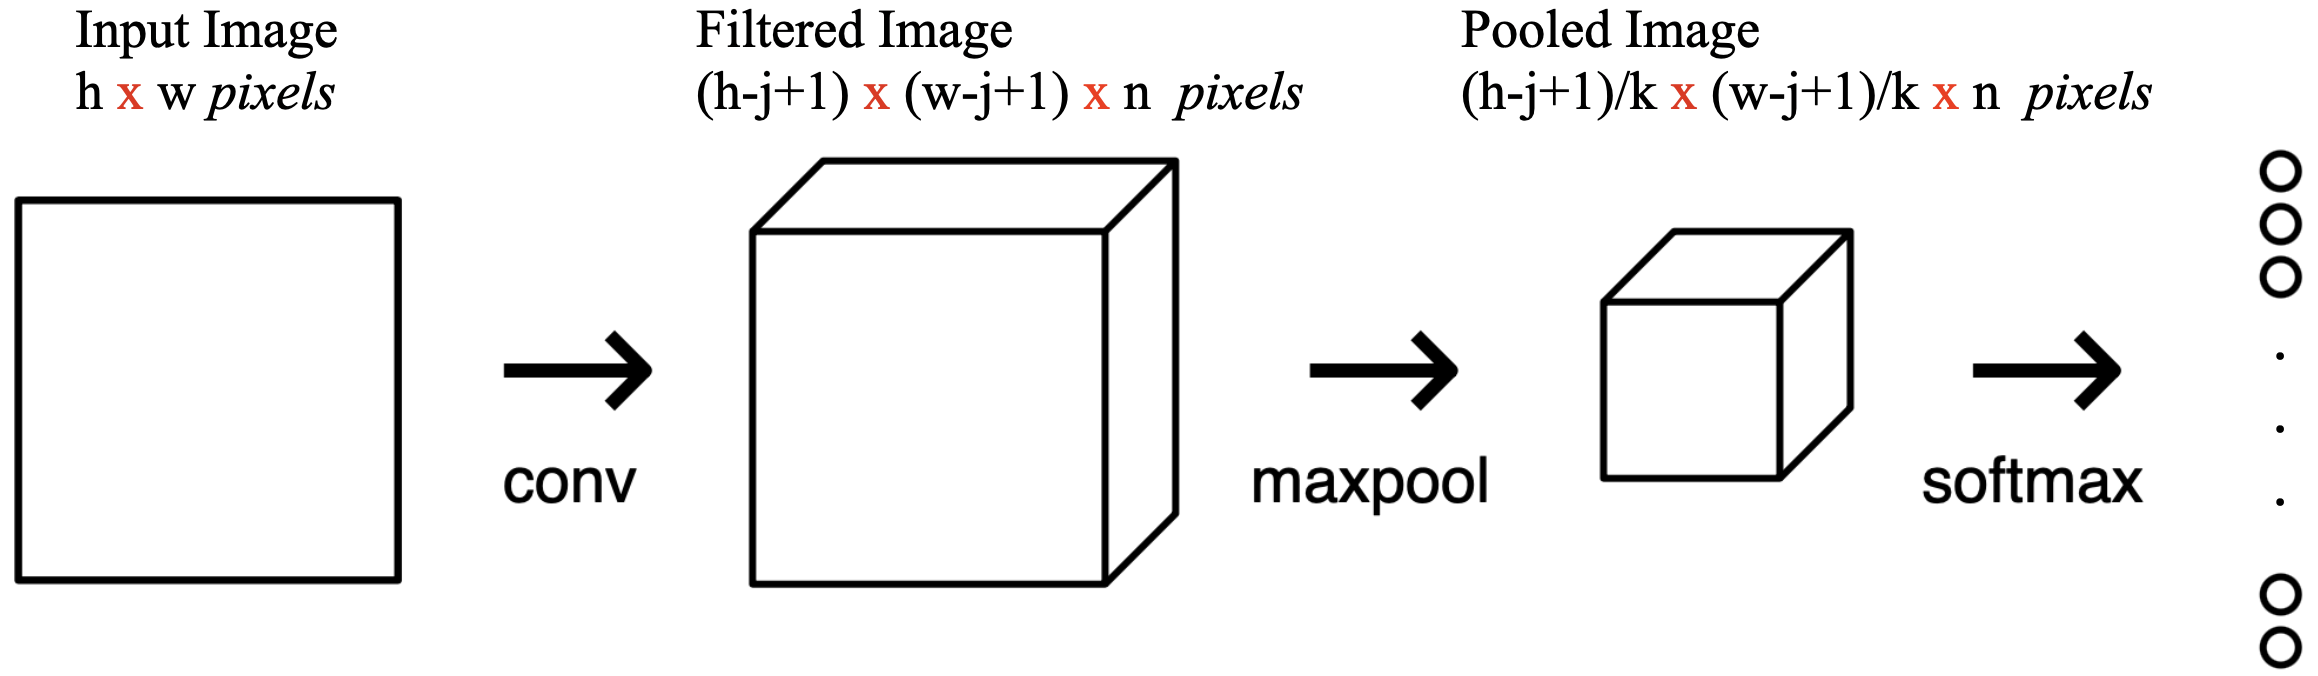
\includegraphics[scale=0.3]{images/CNN_layers.png}
  \caption{Description of image}
\end{figure*}
\indent The Neural Network used in this research consists of 5 layers in total (See Fig.\ref{}). The input and output layers,
represent the raw input image and output model prediction, respectively, and intermediate hidden layers,
\textit{convolutional}, \textit{pooling}, and \textit{activation} layers, each with a specific image analysis task
as described in the subsections below.\\
\subsection{Convolutional Layer}
Briefly describe what the convolutional layer does, its dimensions, and how many filters used and the filter dimentions. Give reference to the online blog you read, \cite{CNNPart1_VZ_2019}
\subsection{Pooling Layer}
Briefly describe what the convolutional layer does, and which specific pooling did you used, e.g., maxpooling?. Give reference to the online blog you read, \cite{CNNPart1_VZ_2019}
\subsection{Activation Layer}
Briefly describe what the activation layer does, and which specific activation layer did you used, e.g., softmax. Maybe you can put the formula of softmax, and introduce mention how the loss is calculated. If you have not
talked about what the the loss, then also give a brief description of what it is (See Ref. \cite{}). For the layer description, give reference to the online blog you read, \cite{CNNPart1_VZ_2019}, and probably also
the article which describes what is softmax. You will need to probably add a new reference to the bibliography to be able to cite the softmax online article, similar to the other citations you have been doing.\\

**IMPORTANT:  Don't worry about putting the details of the math (partial derivatives) that was done to actually carry out the forward/bacpropagation of the neural network.
Just focus on explaining the basics of each layer used, and just mention that once the image passed through the layers, the output was compared to the known result, and
a backpropagation method was done to minimize the loss by determining the optimum parameters. And mention that an epoch consists of a complete forward/backward propagation.
Then, the images were re-analyzed with the updated parameters in subsequent epochs to further optimize the parameters and minimize the loss.  ** You'll probably have to also
give a brief 1-sentence description of what the loss is in a neural network.\\
\indent The data with specific [Q1,Q2,Q3] tunes were simulated using the standard Hall C simulation program (\texttt{mc-single-arm})
and the raw data output was written to a ROOTfile. A separate ROOT C++ script (\texttt{make\_2Doptics.C}) was used to form each of
the six abovementioned 2D focal plane correlations correlations which were stored in a separate ROOTfile as histogram objects.
The 2D histograms were then converted to a 2D pixelated array and stored in binary format (.h5) via a Python code (\texttt{save2binary.py})
array to be read by the Neural Network using Python Keras. Each optics image used was 200x200 pixels and was passed thorugh each of
the hidden layers of the network described in Section 4 of this article.


\section{Results and Discussion}
Summarize results and discuss implications of these results. After spending a great deal of time and energy introducing and arguing the points in the main body of the paper,
the conclusion brings everything together and underscores what it all means. A stimulating and informative conclusion
leaves the reader informed and well-satisfied. A conclusion that makes sense, when read independently from the rest of
the paper, will win praise. \\
\indent The purpose of this research was to teach a machine to recognize optics patterns that would otherwise be
difficult to distinguish by the "human eye". With the help of Keras API, we were able to train and test a CNN
by providing simulated optics data from Jefferson Lab, Hall C.  Each of the six 2D optics correlation was trained with
31 optics tunes, and were able to reach and plateau at an accuracy of ~X \%, and a loss of ~Y \%, in Z epochs of training.
We used 10 test images per each of the six 2D optics correlations, and network was able to correctly predict
each the patterns with at least ~N \% accuracy. The results of the training are shown in Fig.\ref{}

[Here show the plot of Accuracy (and Loss) vs. epochs] to show how the training progresses. \\

The results of the test images is summarized in Table \ref{tab:results}
\begin{table}[h]
	\begin{center}
		\begin{tabular}{llll} % left-aligned, number of l's represent number of headings
                  \hline
                  col1 & col2 & col3 & col4 \\ \hline \hline
	          val1 & val2 & val3 & val4 \\
                  val5 & val6 & val7 & val8 \\
		  \hline 
		\end{tabular}
	\end{center}
	\caption{Caption of table.}
	\label{tab:results}
\end{table}

%dummy text
%\lipsum

\bibliography{references}   
\bibliographystyle{IEEEtran}



\end{document}
